\chapter*{Appendix}
\addcontentsline{toc}{chapter}{Appendix}
\section*{Appendix Index}
\vspace{-8em}

% Adjust indentations before \listofanhang
\abstaendeanhangverzeichnis

\listofanhang
\clearpage
\spezialkopfzeile{Appendix} 

\lstset{
  language=TeX, % define keywords to highlight
  morekeywords={Appendix, anhangteil, anhan},
  breaklines=true,  % Enable line wrapping within the listing
  breakatwhitespace=true, % Breaks only at white space
  postbreak=\mbox{\textcolor{red}{$\hookrightarrow$}\space}, % Optional - for having a symbol at the point where text breaks
  basicstyle=\footnotesize\ttfamily, % for setting the font size/style for the code
  tabsize=2, % sets default tabsize
}


%% ================================== Discussion =======================================

\anhang{Discussion of Tool Evaluation and Weighing}

\anhangteil{Community, Support \& Docs}

This section assesses the level of external support provided for each project. To evaluate this support, we will focus on three distinct aspects and combine them into a single score. Firstly, we will examine the size of the community, as a substantial community often indicates project maturity and the availability of extensive support. As proxies for community size, we will consider two central metrics: the number of stars on GitHub and the quantity of questions on Stack Overflow.

\begin{table}[htb]
    \centering
    \caption[Community Support Data]{Community Support Data\footnotemark}
    \label{tab:community_support} 
    \begin{tabular}{|l|c|c|} 
      \textbf{Project} & \textbf{GitHub Stars} & \textbf{Stack Overflow Questions} \\ 
      Pachyderm  & 6,000   & 6          \\ 
      Argo       & 14,500  & 136        \\ 
      Clasp      & 0       & 0          \\ 
      Snaplogic  & 0       & 57         \\ 
      Airflow    & 32,200  & 10,218     \\ 
      Kubeflow   & 13,100  & 434        \\ 
      Knative    & 4,100   & 204        \\ 
      Luigi      & 16,900  & 346        \\ 
      CWL        & 1,400   & 6          \\ 
   \end{tabular}
\end{table}
\footnotetext{Data taken from GitHub and Stack Overflow on 08.11.2023}

\begin{figure}[htb]
    \centering
    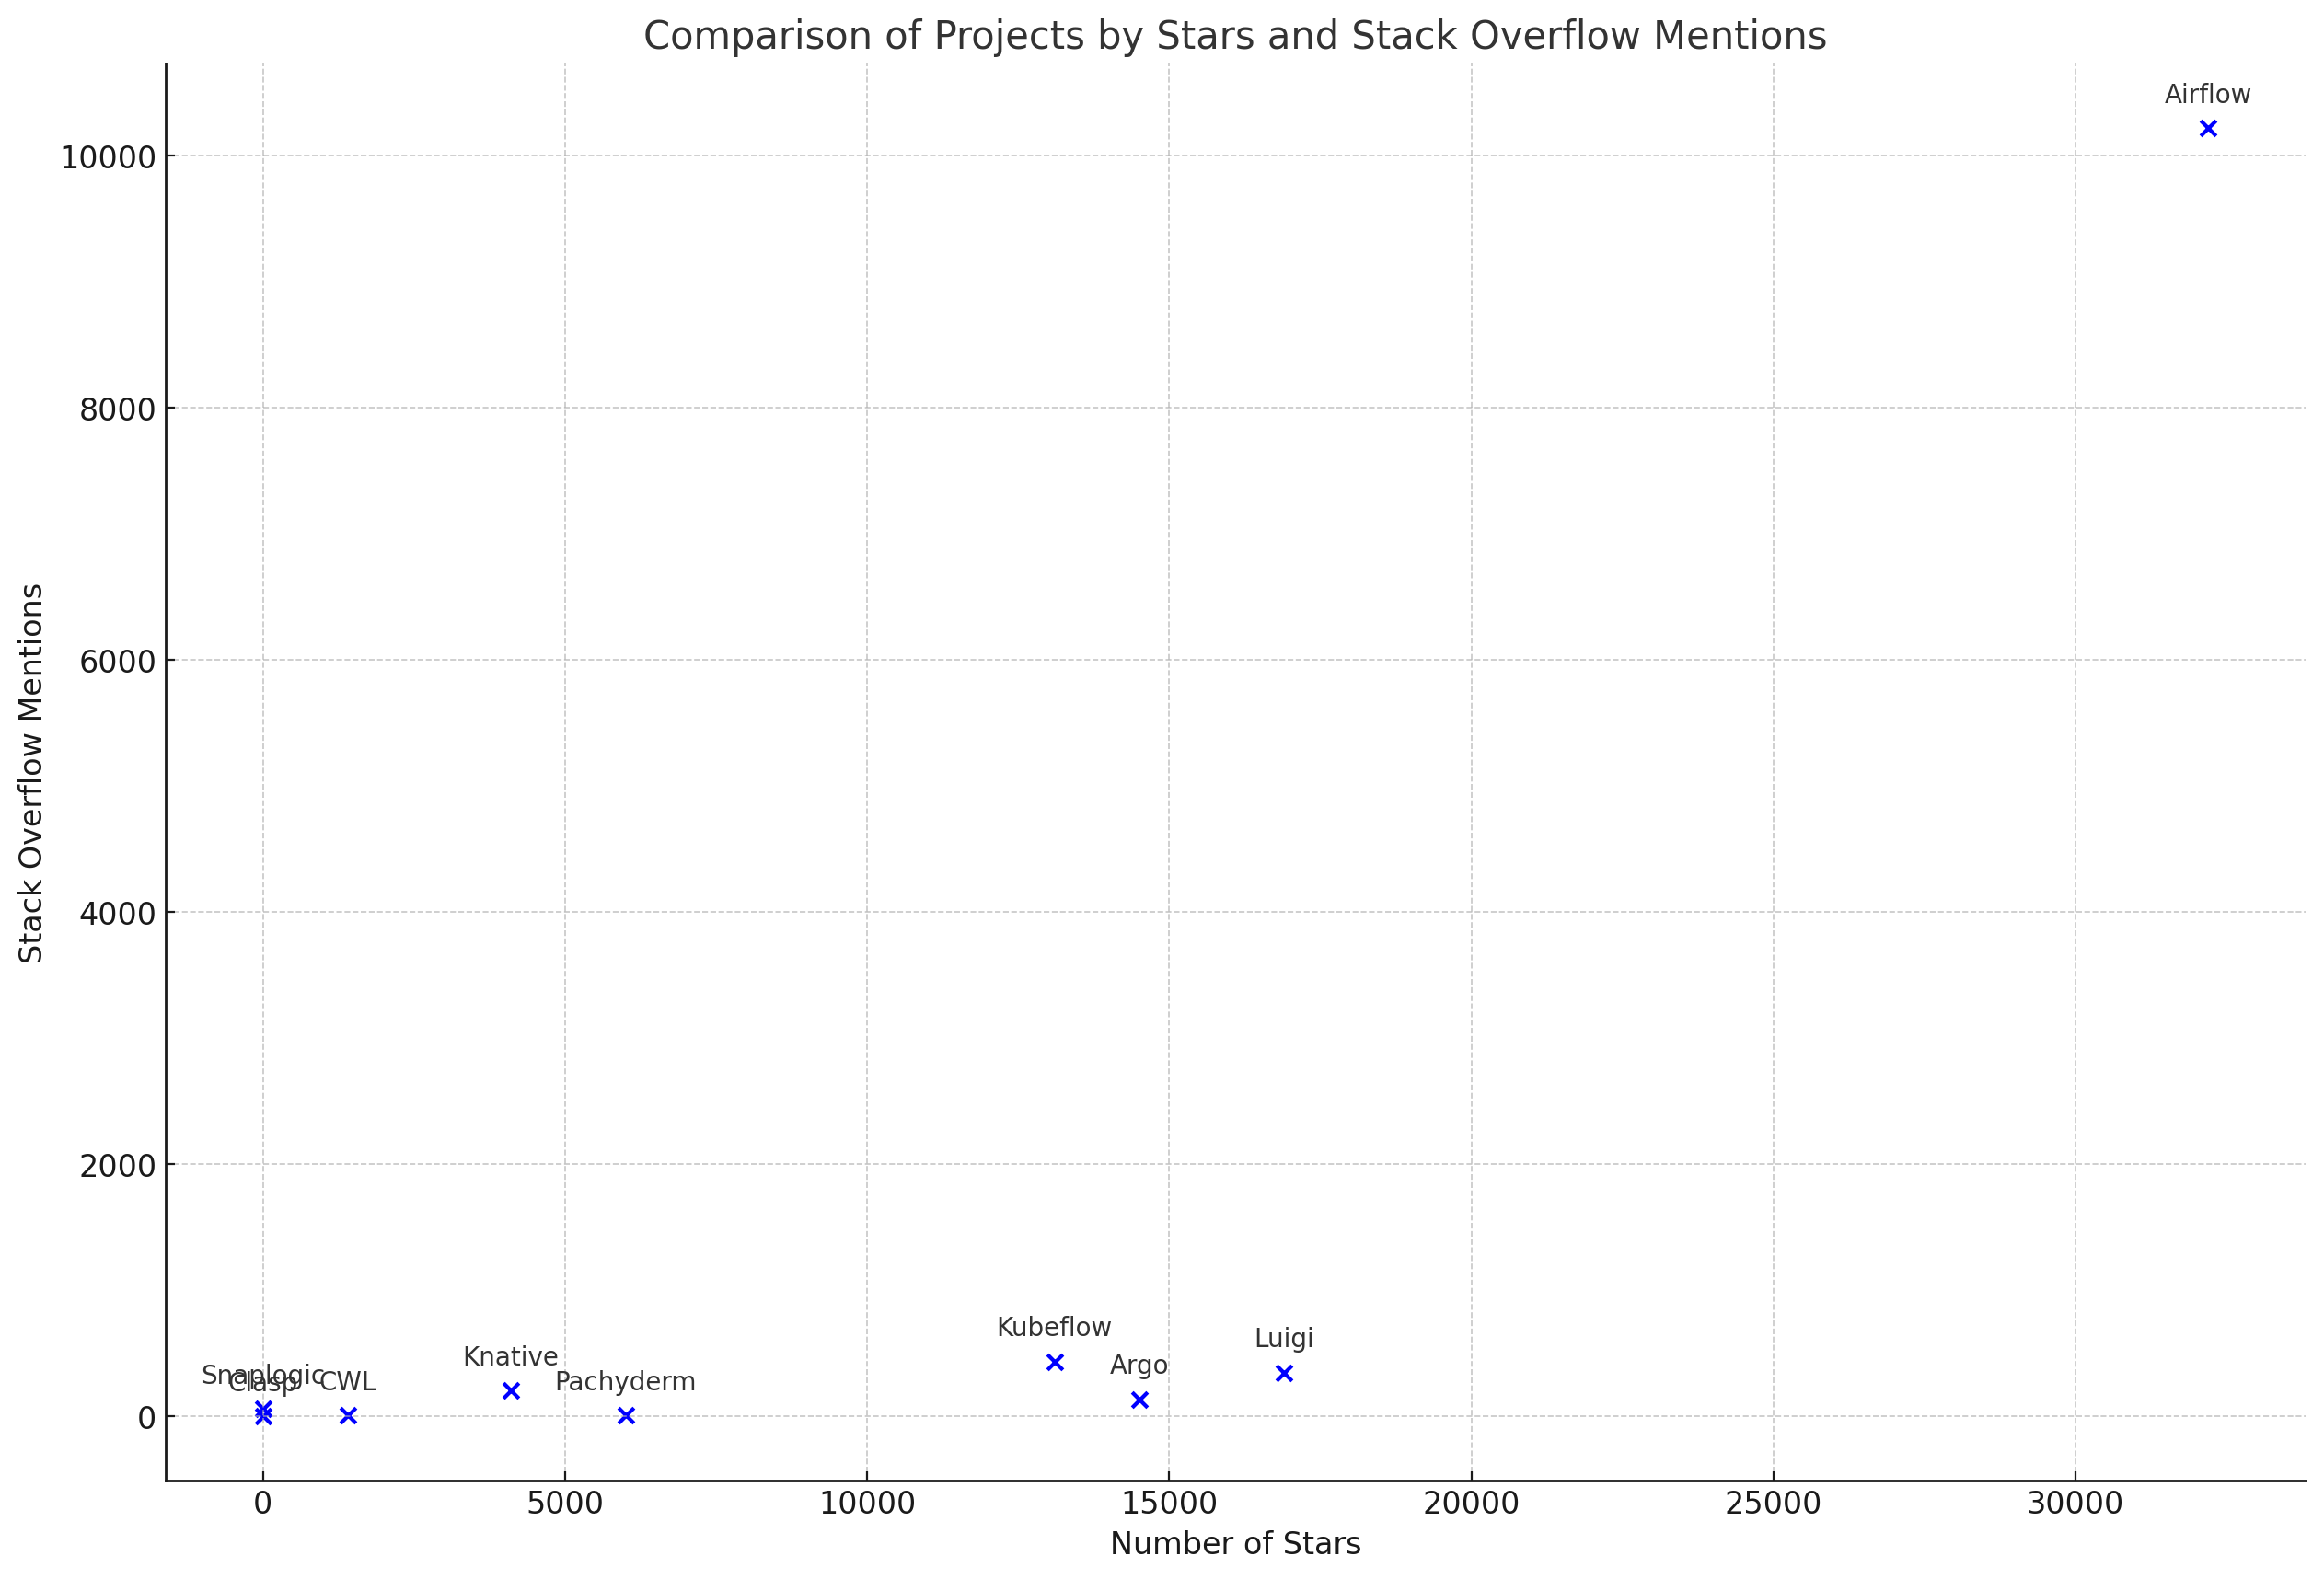
\includegraphics[width=12cm]{graphics/Stars_stackoverflow_comparison.png}
    \caption[Stars and Stack overflow Questions Comparison]{Stars and Stack Overflow Questions Comparison}
    \label{abb:stars_stackoverflow_comparison}
\end{figure}

To gauge the level of support and community engagement surrounding these projects, we have devised a composite score that normalizes and combines the GitHub stars and Stack Overflow questions metrics. The calculation of this score involves the following methodology:

Each project is represented as a point \(P_i = (x_i, y_i)\) in a two-dimensional space, with \(x_i\) and \(y_i\) being the number of GitHub stars and Stack Overflow questions, respectively, for the \(i\)-th project. The composite score \(S_i\) for each project is computed by normalizing these values to a scale of 0-10 and then taking their average.

Additionally, we acknowledge that some commercial tools, as well as certain open-source projects, offer enterprise support, reducing the reliance on the community for assistance. Similarly, projects developed in-house often have access to the original development team for support. Therefore, we will apply a flat bonus of 5 points to the scores of projects offering enterprise support and a flat bonus of 2.5 points to projects developed in-house.

\[S_i = \frac{1}{2} \left( \frac{x_i - \min(x)}{\max(x) - \min(x)} \times 10 + \frac{y_i - \min(y)}{\max(y) - \min(y)} \times 10 \right) + B_i \]

Here, \(\min(x)\), \(\max(x)\), \(\min(y)\), and \(\max(y)\) represent the minimum and maximum values of GitHub stars and Stack Overflow questions across all projects, respectively. The final scores \(S_i\), along with the respective bonuses \(B_i\), provide a comprehensive metric for comparing project popularity, community engagement, and the availability of additional support options, all on the same scale.

\begin{table}[h!]
    \centering
    \begin{tabular}{|l|c|c|c|c|} 
    \hline
        \textbf{Project} & \textbf{Composite Score} & \textbf{Enterprise Bonus} & \textbf{Inhouse Bonus}  & \textbf{Final Score}\\
        \hline
        Airflow & 10.00 & 0 & 0 & 10.00 \\
        Pachyderm & 0.93 & 5 & 2.5 & 8.43 \\
        Snaplogic & 0.03 & 5 & 0 & 5.03 \\
        Luigi & 2.79 & 0 & 0 & 2.79 \\
        Clasp & 0.00 & 0 & 2.5 & 2.5 \\
        Argo & 2.32 & 0 & 0 & 2.32 \\
        Kubeflow & 2.25 & 0 & 0 & 2.25 \\
        Knative & 0.74 & 0 & 0 & 0.74 \\
        CWL & 0.22 & 0 & 0 & 0.22 \\
    \hline
    \end{tabular}
    \caption{Composite scores of Workflow managers, sorted by final score}
    \label{tab:results}
\end{table}

\anhangteil{License}

As discussed in section \ref{crit:license} the tools in consideration should not be too restrictive.
To evaluate the criteria we will employ a 4 bucket system: 
\begin{itemize}
    \item \textbf{Ideal Situation (Score: 10):} 
    This refers to cases where either the tool is in the public domain (and therefore not subject to copyright restrictions) or where our organization possesses a direct ownership or significant influence over the licensing terms.
    This situation provides the most flexibility, allowing for extensive modification, redistribution, and proprietary use without concern for licensing infringements.


    \item \textbf{Permissive License (Score: 7.5):}
    Tools under licenses like MIT, BSD, or Apache 2.0 fall into this category.
    These licenses are highly permissive and generally allow for broad freedom, including modification, distribution, and private use, with minimal restrictions, often limited to liability and warranty.

    \item \textbf{Restrictive or Reciprocal Licenses (Score: 2.5):}
    Licenses such as the GPL or AGPL are more restrictive, requiring any changes to be open-sourced or contributions to be made back to the community.
    These “copyleft” licenses can be problematic in proprietary settings where modifications or integrations need to remain confidential.

    \item \textbf{Unacceptable Licenses (Score: 0):}
    This includes licenses that impose burdensome conditions or high costs, proprietary software where the source code is unavailable, or situations where the licensing terms make it impractical to use within our projects.
    For instance, licenses that mandate the purchase of additional software, restrict certain types of use, or pose potential legal risks would fall into this category.
\end{itemize}

Now we will evaluate the licenses of the tools in question, and assign them a score based on the above criteria.

\begin{itemize}
    \item \textbf{Pachyderm} 
    The licensing model of Pachyderm follows a model which has similarities with the "Open Core model" \footcite{PahcydermPricing2022}.
    Which means that while the core functionalities are published as the "COMMUNITY EDITION" with a permissive source-available License (Apache License 2.0) \footcite{PachydermLICENSEMaster}.
    Functionality like \ac{SSO} or the ability to create more than 16 pipelines are part of a different distribution under a Commercial License.

    But in our case this is of no concern, as the startup behind the Pachyderm software, including its \ac{IP} was acquired by \ac{HPE}.
    Giving us a free hand to modify without needing to worry.

    \item \textbf{Argo}Argo's adoption of the Apache License 2.0 \footcite{ArgocdLICENSEMaster} aligns with common practices for open-source projects, affording users considerable freedom. This permissive license simplifies the use, modification, and redistribution of the software, an aspect that's particularly beneficial for collaborative development or integration into proprietary software. Given our requirements and operational context, this offers us the flexibility needed for adaptation and potential enhancements without stringent restrictions, streamlining any developmental efforts we undertake with Argo.
    \item \textbf{\ac{CLASP}} is not a published software and therefore not under any specific license.
    But similar considerations as the ones of Pachyderm apply here as well, as it is an internal project the \ac{IP} also completely belongs to \ac{HPE}

    \item \textbf{Snaplogic} is an entirely commercial product which does not provide insight into nor the right to modify their Software \footcite{SnapLogicMasterSubscription}.
    But as they might agree this is not a total knockout criterion for this entire project, but in regard to the licensing it will be weighted with 0.
    \item \textbf{Airflow} is licensed under the Apache License 2.0. \footcite{LicenseAirflowDocumentation}
    \item \textbf{Kubeflow} is licensed under the Apache License 2.0. \footcite{KubeflowLICENSEMaster}
    \item \textbf{Knative} is licensed under the Apache License 2.0. \footcite{KnativeDocsLICENSE}
    \item \textbf{Luigi} is licensed under the Apache License 2.0. \footcite{LuigiLICENSEMaster}
    \item \textbf{CWL} is licensed under the Apache License 2.0. \footcite{CwlutilsLICENSEMain}
    
\end{itemize}

\anhangteil{Strategic alignment}

When considering the strategic alignment within the context of \ac{HPE} the goal is to ensure that the tool can be used in combination with or as extension to the Products \ac{HPE} is offering.
Tools that have been developed by the company in the first place or have been acquired by \ac{HPE} must be of a high strategic value to the company, as otherwise they would not have been developed or acquired in the first place.

This is especially true for Pachyderm, as it has been acquired in 2023 \footcite{HewlettPackardEnterprise} as part of their realignment towards hybrid cloud provider.
The eight years since the development of \ac{CLASP} in 2015 \footcite{sayersCLoudApplicationServices2015} the priorities of somewhat shifted, its concept is still relevant and was originally developed by the labs to fill a strategic gap.

While some of these tools might have been used in other projects, been contributed to by \ac{HPE} employees or are supported on the Ezmeral platform, they are not part 
of the core product portfolio and therefore not of strategic importance.

One thing that would have to be considered is the way one would make oneself dependant of the company, as \ac{HPE} would have to enter into negotiations with the company behind Snaplogic, 
this state of dependency an the need to find a compromise would be a strategic disadvantage.

Therefore the following scores have been assigned:

\begin{table}[htb]
  \centering
  \caption{Strategic Alignment Scores}
  \begin{tabular}{|l|c|} 
    \textbf{Project} & \textbf{Strategic Alignment} \\
    Pachyderm  & 10   \\
    \ac{CLASP}       & 7.5  \\
    Argocd       & 2.5  \\
    Snaplogic      & 0          \\
    Airflow      & 2.5          \\
    Kubeflow      & 2.5          \\
    Knative      & 2.5          \\
    Luigi      & 2.5          \\
    CWL      & 2.5          \\
  \end{tabular}
\end{table}

\anhangteil{Ease of Use}

\anhangteil{Maturity}

The evaluation of the tools is centrally based on their open source repositories, as this is the most accessible and transparent source of information.
In order to evaluate the maturity of the tools, we will look at the age, the number of commits, the ratio of commits to age, the number of closed issues and the ratio of closed issues to open issues.
We will then combine these metrics into a single score, which will be used to evaluate the maturity of the tools. Products like Snaplogic, which are not open source,
as they are a commercial product it is to be expected that they are somewhat mature, as they are already being used in production environments and are used by many companies.


\begin{table}[htb]
  \centering
  \label{tab:maturity_data}
  \begin{tabular}{|l|c|c|c|c|c|}
    \hline
    \textbf{Project} & \textbf{Age (Days since 08.11.2023)} & \textbf{Commits} &  \textbf{ Open Issues} & \textbf{Closed Issues} \\
    \hline
    Pachyderm  & 3352 & 22143 & 889 & 2387  \\
    Argo      & 2098 & 6047  & 2693 & 4161 \\
    Airflow    & 3131 & 22026 & 762 & 7467 \\
    Kubeflow   & 2168 & 2514  & 178 & 3615 \\
    Knative    & 2113 & 8531  & 202 & 4332 \\
    Luigi      & 4066 & 4088  & 93  & 879  \\
    CWL        & 2954 & 4512  & 421 & 358  \\
    \hline
 \end{tabular}
 \caption[Maturity Data]{Maturity Data\footnotemark}
\end{table}
\footnotetext{Data taken from GitHub on 08.11.2023}


How these values compare to each other in normalized form is shown in the following graphs:

\begin{figure}[H]
  \centering
  \begin{minipage}{.5\textwidth}
    \centering
    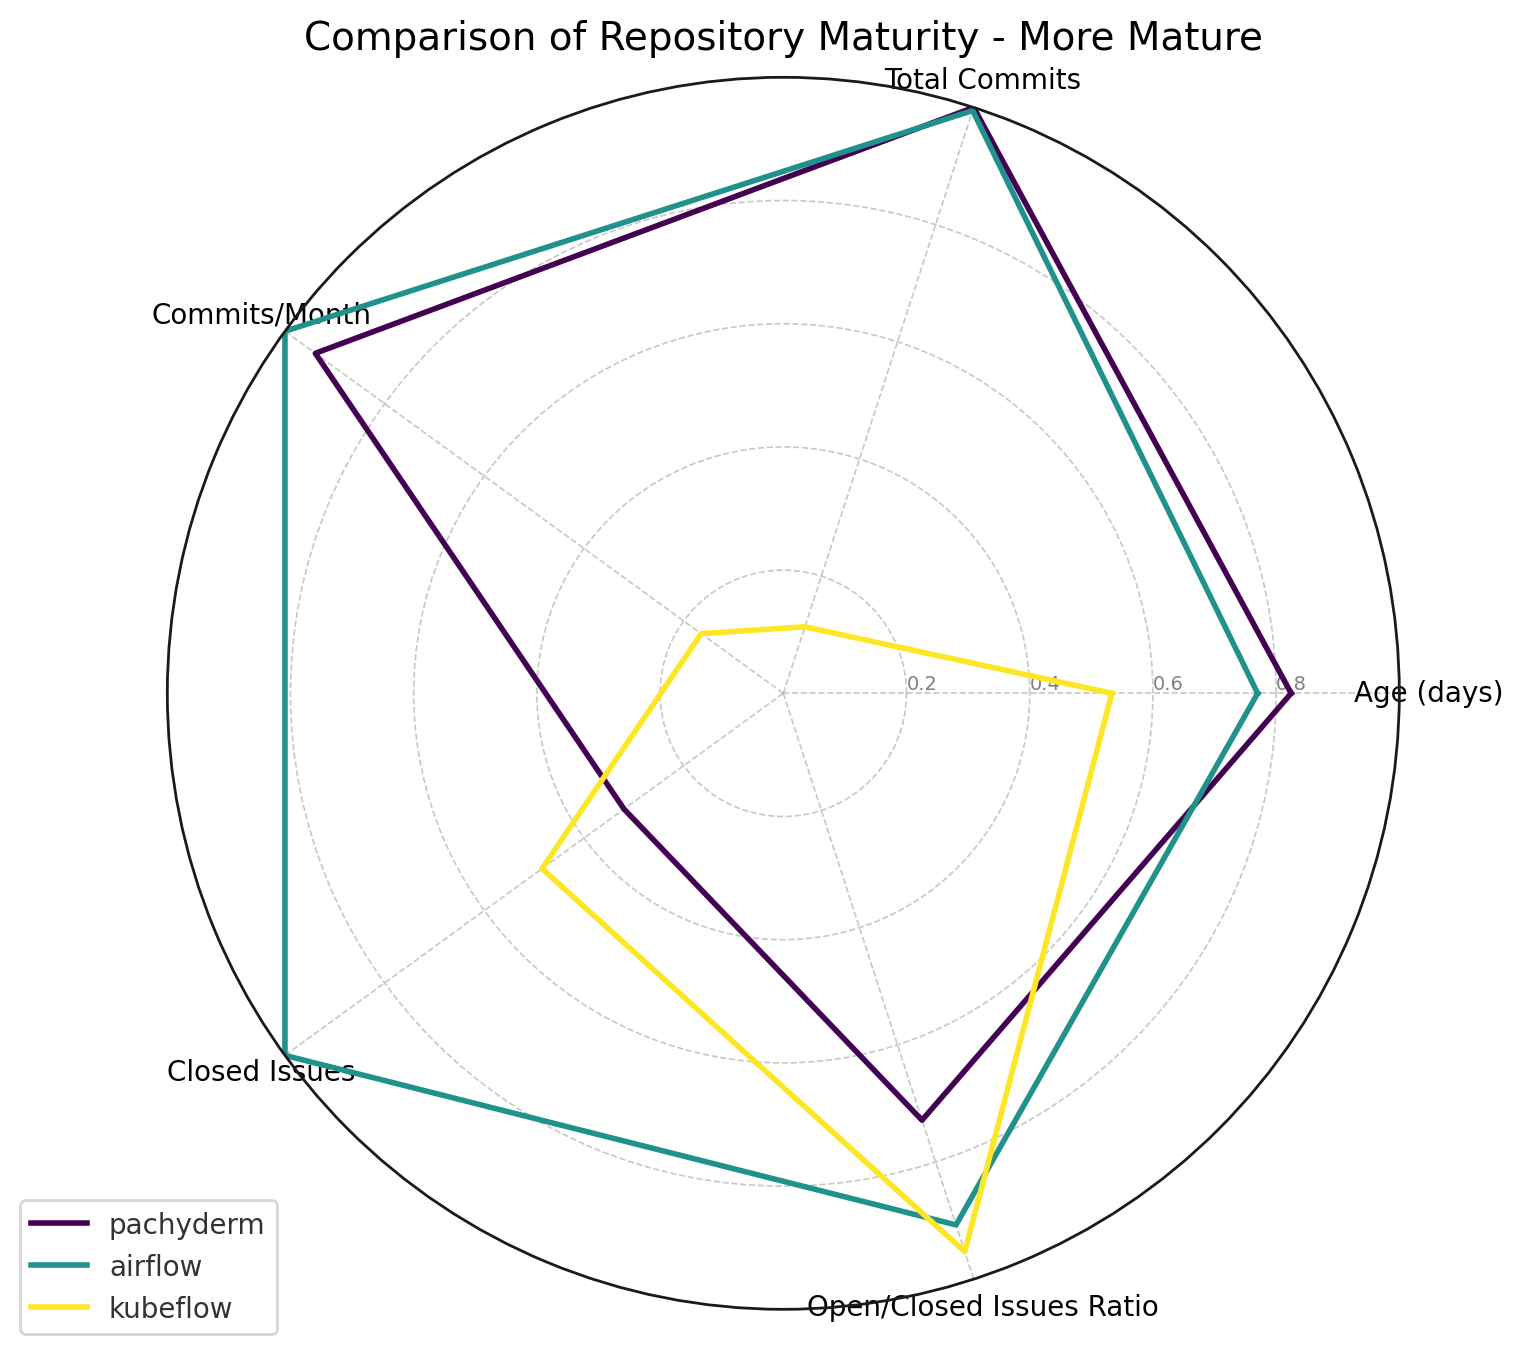
\includegraphics[width=6cm]{graphics/Maturity_graph_larger.png}
    \caption[Maturity Metric comparison (higher rated projects)]{Maturity Metric comparison}
    \label{abb: maturity_metric_comparison_larger}
  \end{minipage}%
  \begin{minipage}{.5\textwidth}
    \centering
    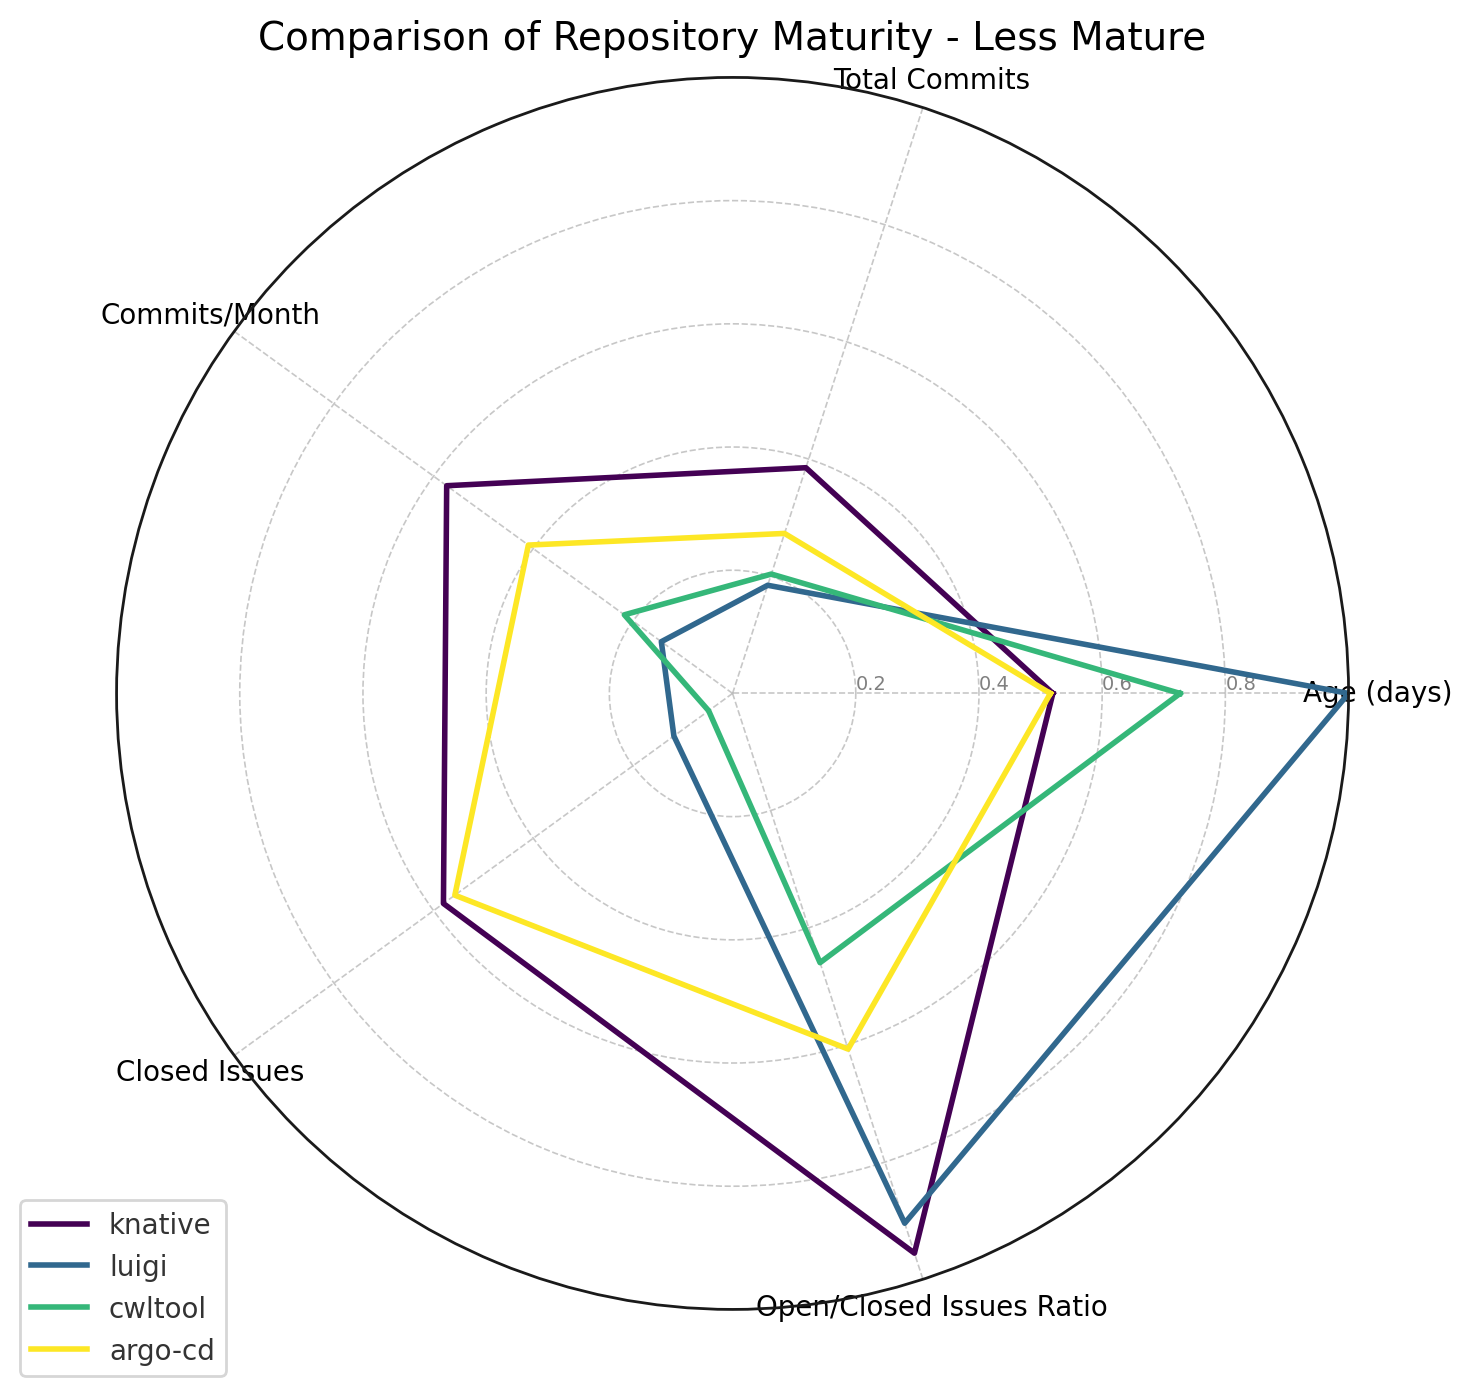
\includegraphics[width=6cm]{graphics/Maturity_graph_smaller.png}
    \caption[Maturity Metric comparison (lower rated projects)]{Maturity Metric comparison}
    \label{abb: maturity_metric_comparison_smaller}
  \end{minipage}
\end{figure}


The combined maturity score for each tool is calculated as follows:


\begin{itemize}
  \item Age (days): Current Date - Created Date
  \item Commits/Month: Total Commits / (Age in months)
  \item Open/Closed Issues Ratio: Closed Issues / (Open Issues + Closed Issues)
  \item Normalized Metrics: Each metric is normalized by dividing by the maximum value among all repositories.
  \item Combined Maturity Score: Average of normalized metrics, scaled to a 1-10 range as \( 1 + (9 \times \text{average}) \).
\end{itemize}

\begin{table}[htb]
  \centering
  \caption{Maturity Scores}
  \begin{tabular}{|l|c|} 
    \textbf{Project} & \textbf{Maturity Score} \\
    Pachyderm  & 7.86   \\
    Argo       & 5.2  \\
    Airflow    & 9.41  \\
    Kubeflow   & 5.05  \\
    Knative    & 6.43  \\
    Luigi      & 5.23  \\
    CWL        &  3.98 \\
  \end{tabular}
\end{table}

\anhangteil{Cost}

This section aims to compare the relative cost of the products in relation to each other.
We previously factored in the enterprise features, so when enterprise support is available and applicable we will take this into consideration.
Here we have three categories of products first those which are completely free and without any enterprise support,
secondly those which are free but offer enterprise support and lastly those which operate on a subscription basis.
To address various cost models, we classify the tools into the following categories:

\begin{enumerate}
  \item \textbf{Open-source and Community-Supported Tools (No Cost):} Free tools, typically open-source, relying on a community for maintenance.
  \item \textbf{Open-source with Optional Enterprise Support (Variable Cost):} Open-source with paid enterprise support offering advanced features by the developing team.
  \item \textbf{Commercial Products (Subscription-Based Cost):} Tools that require ongoing payment for use depending on the level of service and feature access.
\end{enumerate}


\begin{table}[htb]
  \centering
  \caption{Scores Based on Cost}
  \label{tab:cost_scores}
  \begin{tabular}{|l|c|}
    \hline
    \textbf{Project} & \textbf{Cost Score} \\
    \hline
    Airflow        &  10 \\
    Pachyderm      &   6  \\
    Snaplogic      &   3  \\
    Luigi          &  10 \\
    CLASP          &  10 \\ 
    Argo           &  10 \\
    Kubeflow       &  10 \\
    Knative        &  10 \\
    CWL            &  10 \\
    \hline
  \end{tabular}
\end{table}




%% ============================== Diagrams =====================================


\anhangteil{Lookup table weighing functions}
\begin{figure}[H]
  \centering
  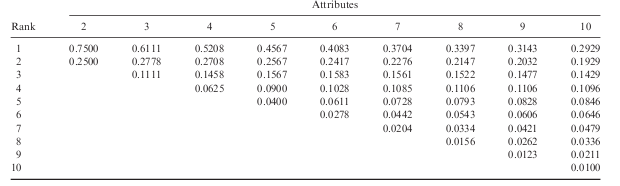
\includegraphics[width=16cm]{graphics/ROC_weights.png}
  \caption[ROC weights]{ROC weights \footnotemark}
  \label{abb:Roc_weights}
\end{figure}
\footnotetext{Taken from: \cite{robertsWeightApproximationsMultiattribute2002a}}


\begin{figure}[H]
    \centering
    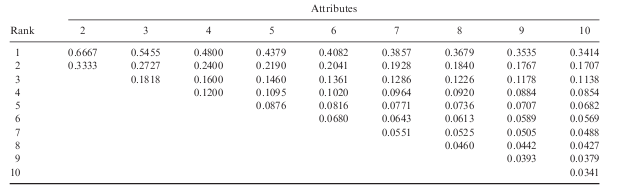
\includegraphics[width=16cm]{graphics/RR_weigths.png}
    \caption[RR weights]{RR weights \footnotemark}
    \label{abb:RR_weights}
  \end{figure}
  \footnotetext{Taken from: \cite{robertsWeightApproximationsMultiattribute2002a}}
  
\begin{figure}[H]
    \centering
    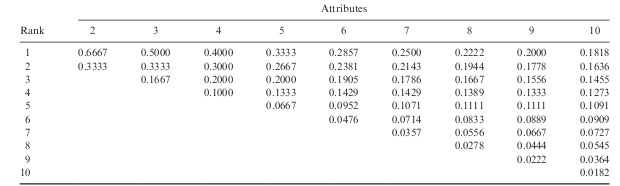
\includegraphics[width=16cm]{graphics/RS_weigts.png}
    \caption[RS weights]{RS weights \footnotemark}
    \label{abb:RS_weights}
  \end{figure}
  \footnotetext{Taken from: \cite{robertsWeightApproximationsMultiattribute2002a}}
  


\anhangteil{Pipeline Communication Swim Lane Diagram}
\begin{figure}[H]
  \centering
  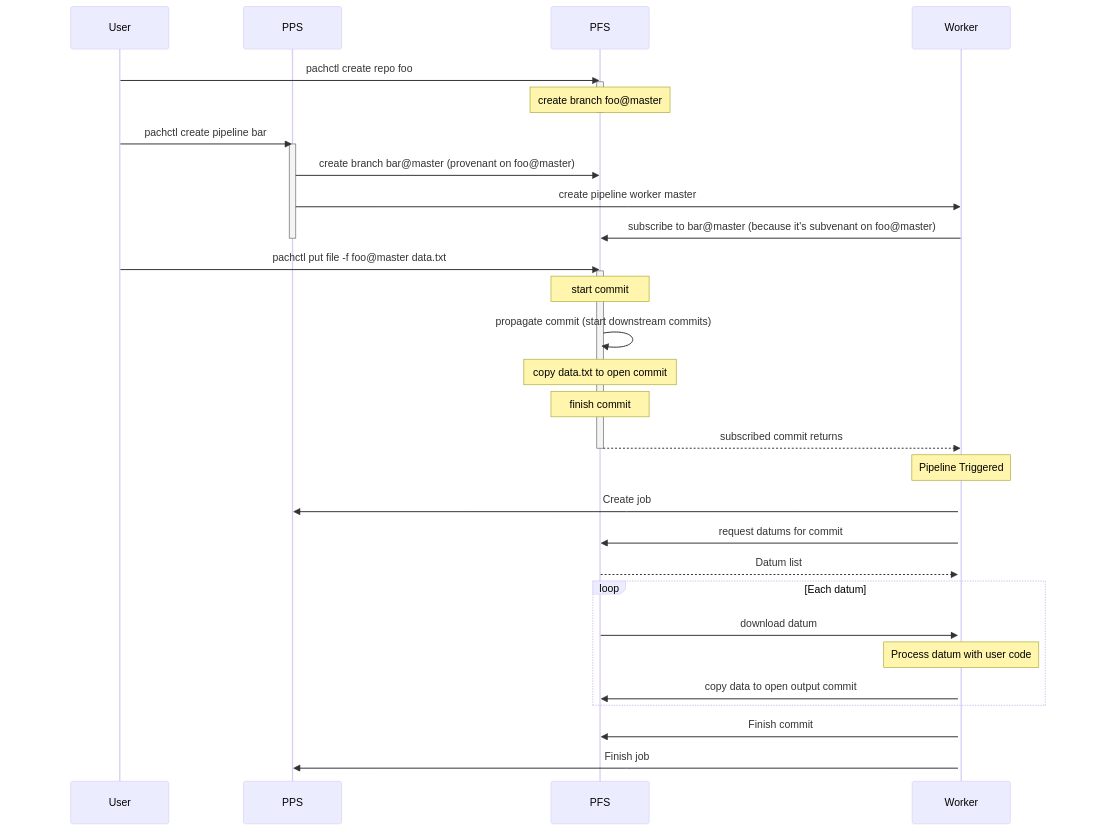
\includegraphics[width=14cm]{graphics/pipeline_communication_sld.png}
  \caption[Swim lane Diagram of the communication between the user and Pachyderm]{Swim lane Diagram of the communication between the user and Pachyderm\footnotemark}
  \label{abb:pipeline_communication_sld}
\end{figure}
\footnotetext{Taken from: \cite{IntroPipelines2023}}


\newpage
\anhang{Diagrams}


\anhangteil{Jenkins Pipeline Diagram}
\begin{figure}[H]
  \centering
  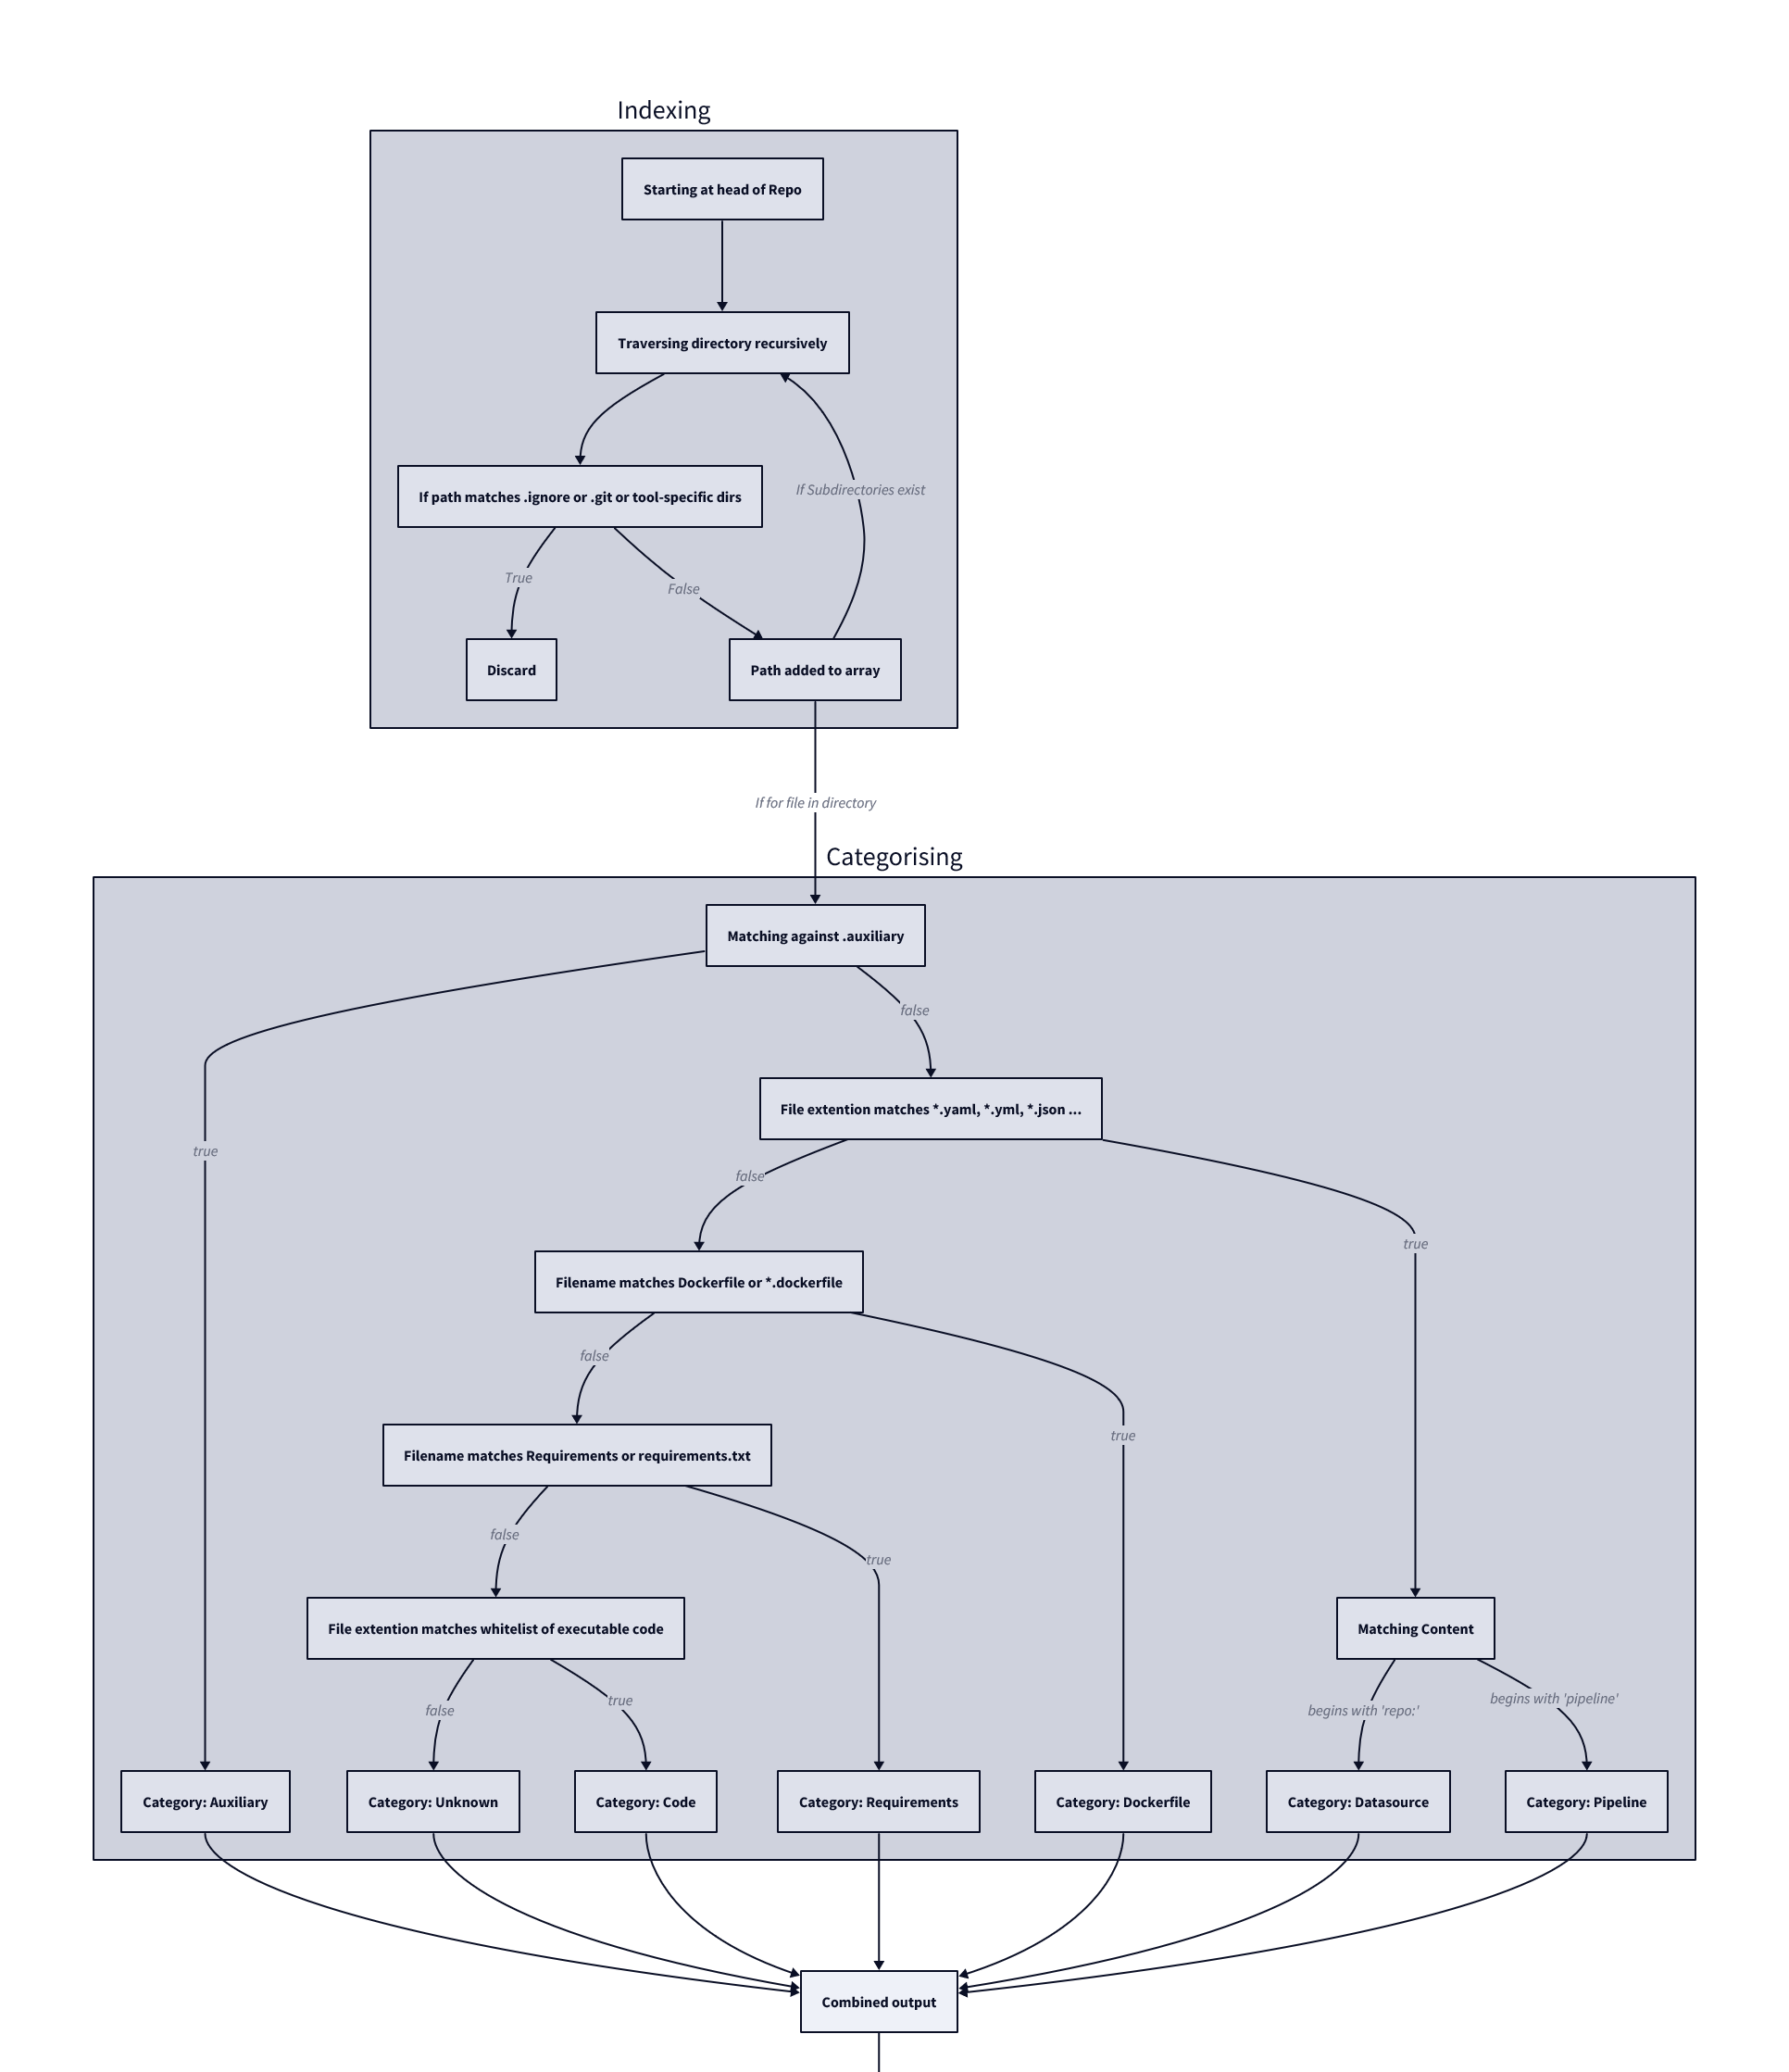
\includegraphics[width=16cm]{graphics/flowchart_pipeline_upper.png}
  \caption{Flowchart of the Jenkins Pipeline}
  \label{abb:flowchart_pipeline_upper}
\end{figure}


\begin{figure}[H]
  \centering
  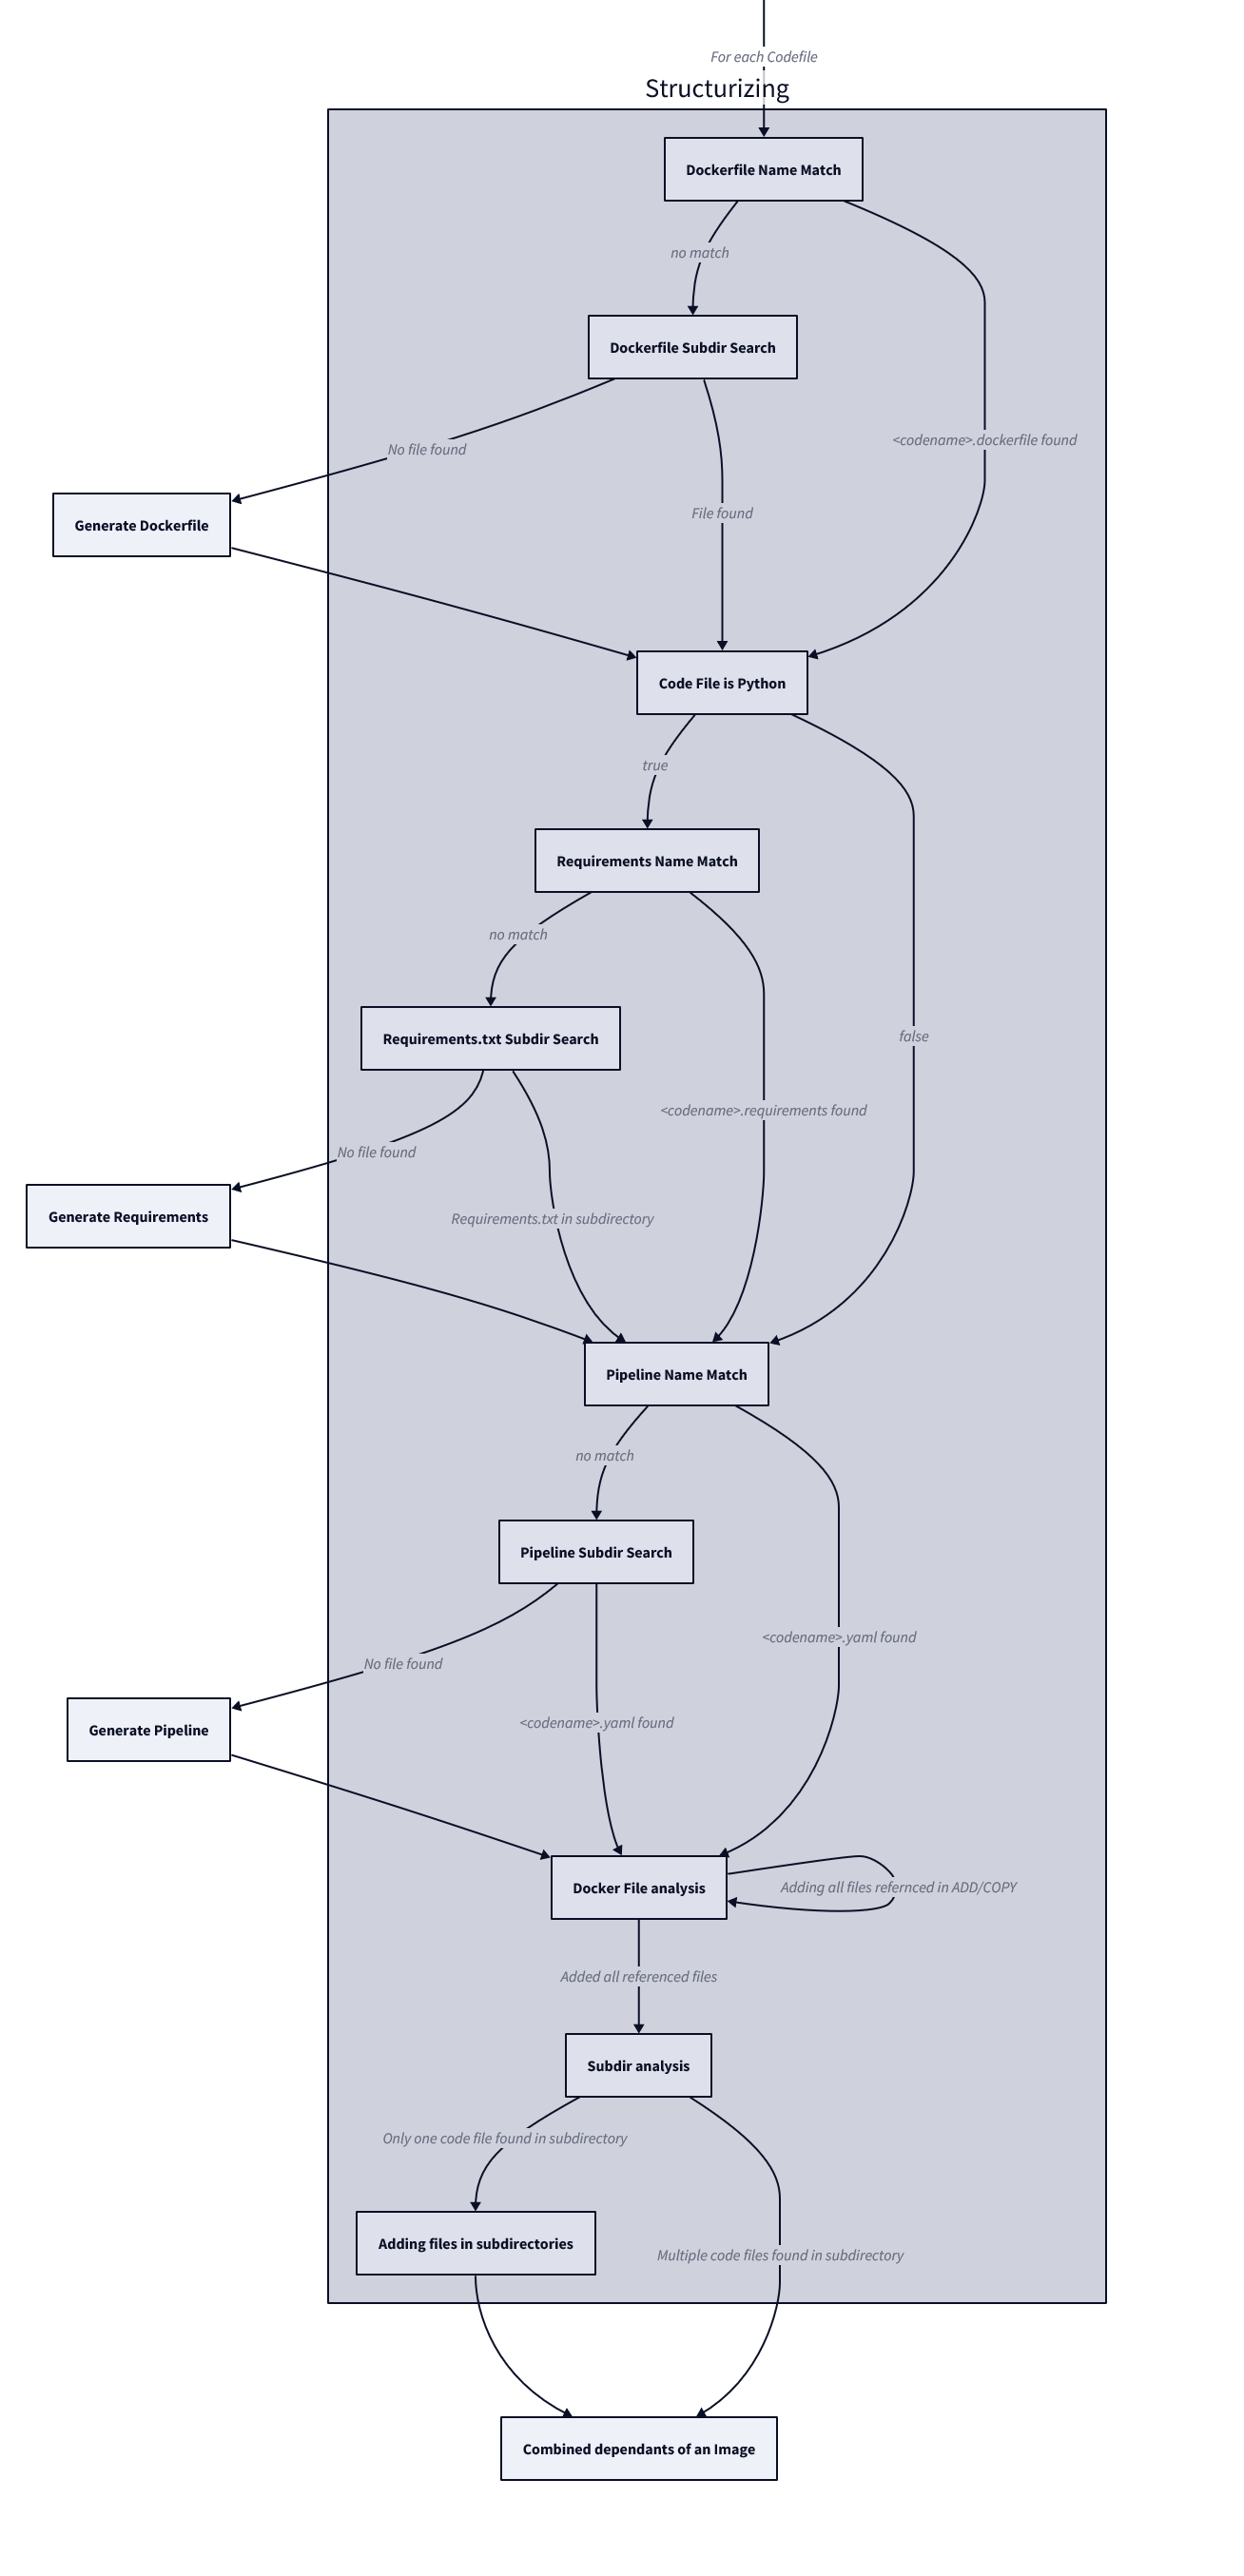
\includegraphics[width=12cm]{graphics/flowchart_pipeline_lower.png}
  \caption{Continued flowchart of the Jenkins Pipeline}
  \label{abb:flowchart_pipeline_lower}
\end{figure}

\newpage


%% ================================ README and Installation instuctions =======================================

\anhang{Minikube installation instructions}
\label{appendix:minikube_installation_instructions}
\lstinputlisting{../quellen/minikube_installation_instructions.md}

\anhang{CI/CD installation instructions}
\label{appendix:cicd_installation_instructions}
\lstinputlisting{../../Project/Kubernetes_Setup/ci_cd/README.md}
